\graphicspath{{chapters/03/media/}}
\chapter{Processamento dei dati}
\label{cha:processamento}
Dopo aver definito in \S\ref{cha:intro} l'obiettivo di questo progetto si deve definire una pipeline che, da dati di sequenziamento di RNA e di \emph{WES}\footnote{SEMPRE DEFINITO NEL CAPITOLO 1} sia in grado di fornire le istanze di espressione allelo-specifica.
Questa pipeline viene definita basandosi su quella presentata in \cite{ase_pipeline} e si compone pertanto di tre fasi principali:
\begin{enumerate}
	\item Pre-processamento e allineamento dei dati di RNA-seq, con eventuale deduplicazione e ricalibrazione.
	\item Analisi di dati \emph{WES} in modo da ottenere una lista di possibili SNP esonici da considerare.
	\item Ottenimento dei dati di sbilanciamento allelico.
\end{enumerate}
La figura \ref{fig:proj_pipeline} \`e una visualizzazione della pipeline e dei tool utilizzati.\\
Essendo infine che questo lavoro prevede il processamento di un gran numero di file, unito al fatto che i tool utilizzzati sono stati implementati con una integrazione con le pipe di unix e con la possibilit\`a di essere eseguiti in multi-threading \`e stato di fondamentale importanza l'utility parallel \cite{parallel}.
In particolare nel caso di STAR\footnote{\S\ref{subsec:star}} \`e stato notato una diminuzione lineare delle performance per thread del tool.
L'abbassamento delle performance \`e stato risolto grazie a parallel, lanciando pi\`u istanze parallele del tool, ognuna di esse con pochi thread.
Si nota pertanto che parallel permette non solo un'elegante implementazione della pipeline, ma fornisce un livello di controllo tale da sfruttare completamente la potenza computazionale disponibile, riducendo in questo modo il tempo globale di esecuzione.


  \begin{figure}[H]
    \label{fig:proj_pipeline}
    \centering
    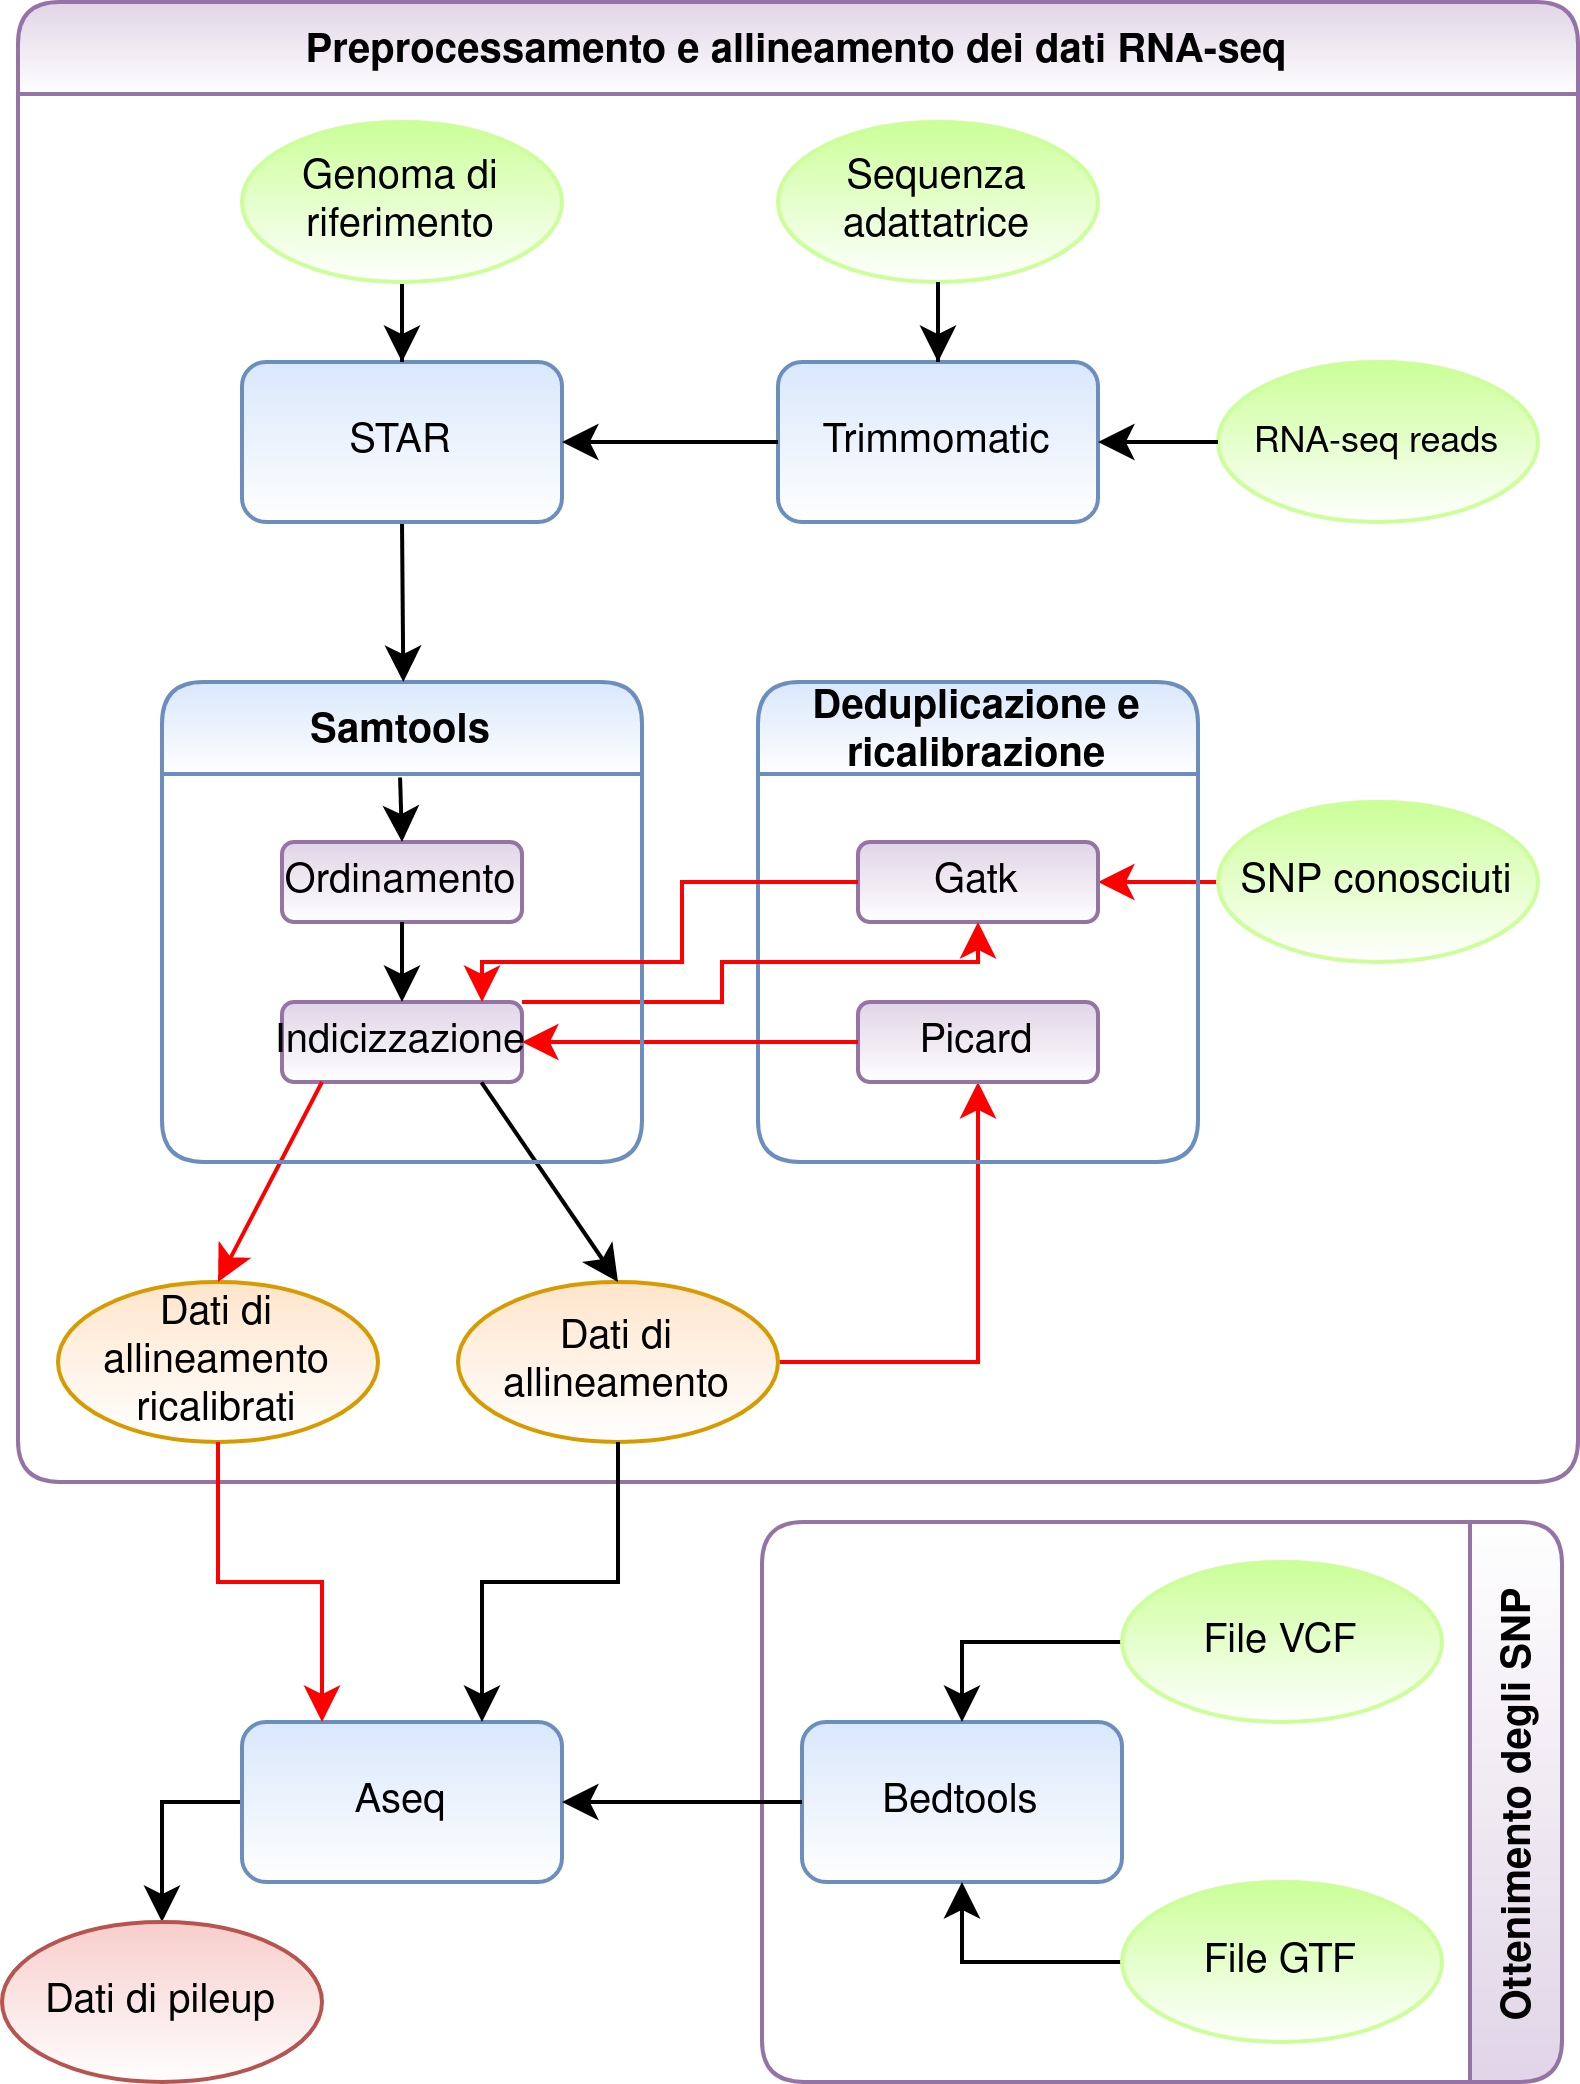
\includegraphics[scale=0.2]{pipeline.png}
    \caption{Pipeline}
  \end{figure}

  \section{Pre-processamento e allineamento dei dati RNA-seq}
  \label{sec:pre_all_rna_seq}
  Il primo passo della pipeline appenda definita \`e il pre-processamento e l'allineamento dei dati RNA-seq.
  L'input della pipeline sono dei file \emph{FASTQ}, ovvero file di testo che contengono i dati di sequenziamento raccolti in laboratorio tipicamente compressi.
  Questi file vengono modificati dai tool Trimmomatic, Star e Samtools in modo da produrre un output gi\`a utilizzabile per ottenere i dati di sbilanciamento allelico.
  Opzionalmente l'output pu\`o subire ulteriori modifiche prima di passare alla prossima fase: in particolare pu\`o essere deduplicato e ricalibrato.
	
  	\subsection{Trimmomatic}
	Trimmomatic \cite{trimmomatic} \`e il primo tool ad essere utilizzato.
	Il suo obiettivo \`e quello di eliminare dalle reads la sequenza adattatrice, o suoi frammenti, utilizzata per rendere possibile il sequenziamento.
	Essendo le RNA-seq fornite a single-ends\footnote{Spiega cosa sono} viene utilizzata la simple mode del tool.
	Questa scansiona ogni read\footnote{Non so se metterla in italiano} dalla terminazione $5'$ alla $3'$ per determinare la presenza della sequenza adattatrice.
	Utilizza il mdetodo ``seed and extend'' per trovare corrispondenze iniziali, anche non perfette, tra la read e la sequenza adattatrice.
	Successivamente svolge un allineamento locale e se questo ha uno score maggiore di una soglia viene rimosso insieme alla porzione successiva ad esso.
	Questa modalit\`a permette di identificare ogni sequenza adattatrice in ogni luogo della read a patto che l'allineamento sia abbastanza lungo e la read abbastanza accurata.
	Si nota per\`o come nelle regioni dove solo una corta corrispondenza parziale \`e possibile come alle estremit\`a della read e pertanto i contaminanti non possono essere identificati attendibilmente.
	Oltre alla rimozione delle sequenze adattatrici Trimmomatic tronca un'estremit\`a secondo un algoritmo di filtraggio secondo qualit\`a.
	Tra i metodi forniti dallo strumento \`e stato utilizzato quello del ``sliding window quality filtering'':
	scansiona la read dal $5'$ e rimuove la terminazione $3'$ quando la qualit\`a media di un gruppo di basi scende sotto una soglia specificata.



  \section{Dati disponibili}
  \label{sec:dati}

    \subsection{Sequenze biologiche}
    \label{subsec:fastq}

    Descrizione dei fastq.

    \subsection{Genoma di riferimento}
    \label{subsec:star-gen}
    Descrizione del genoma di riferimento.

    \subsection{Variant call}
    \label{subsec:vcf}
    Descrizione dei vcf.

    \subsection{Struttura dei geni}
    \label{subsec:gtf}
    Descrizione del gtf.

  \section{Troncatura e allinamento}
  \label{sec:trimm_star}
  Descrizione del processo e perch\`e viene fatto.

    \subsection{Troncatura}
    \label{subsec:trimm}
    Trimmomatic, cosa fa come \`e stato usato.

    \subsection{Allineamento}
    \label{subsec:star}
    STAR, cosa fa come \`e stato usato.

    \subsection{Ordinamento}
    \label{subsec:sorting}
    SAMTOOLS SORT cosa fa come \`e stato usato.

    \subsection{Indicizzazione}
    \label{subsec:indexing}
    SAMTOOLS index cosa fa come \`e stato usato.

  \section{Deduplicazione, riallinamento e recalibrazione}
  \label{sec:recalibration}
  Descrizione del processo e perch\`e viene fatto

    \subsection{Deduplicazione}
    \label{subsec:dedup}
    Come sopra.

    \subsection{Riallineamento e recalibrazione}
    \label{subsec:recalibration}
    Come sopra.

  \section{Ottenere le varianti alleliche}
  Intersezione tra VCF e GTF.

  \section{Ottenere i dati delle frazioni alleliche}
  \label{sec:aseq}
  ASEQ cosa fa come viene usato.


    \subsection{Filtrare le frazioni alleliche}
    \label{subsec:filter}
    Condizioni di filtraggio per i risultati di ASEQ.

  \section{Ottenere gli SNP nel 3'-UTR}
  \label{sec:threeprime}
  Filtraggio del gtf e intersezione con i VCF
